\begin{frame}{SEMFEM}
  \begin{itemize}
    \item Precondition high-order system using low-order discretizations with coinciding nodes.
    \item Orszag \footcite{parter_spectral_1979} demonstrated $\kappa(\mathbf M^{-1} \mathbf A) \sim \pi^2/4$ scaling for second-order Dirichlet problems.
    \item Bello-Maldonado and Fischer \footcite{bello-maldonado_scalable_2019} proposed one-per-vertex scheme.
    \begin{itemize}
      \item{
        Same, single V-cycle AmgX \footcite{naumov_amgx_2015}, damped Jacobi ($\omega = 0.9$).
        }
    \end{itemize}
    \item Other approaches exist, such as Pazner \footcite{pazner2020efficient}.
  \end{itemize}
  \vspace{-0.35cm}
  \begin{figure}
    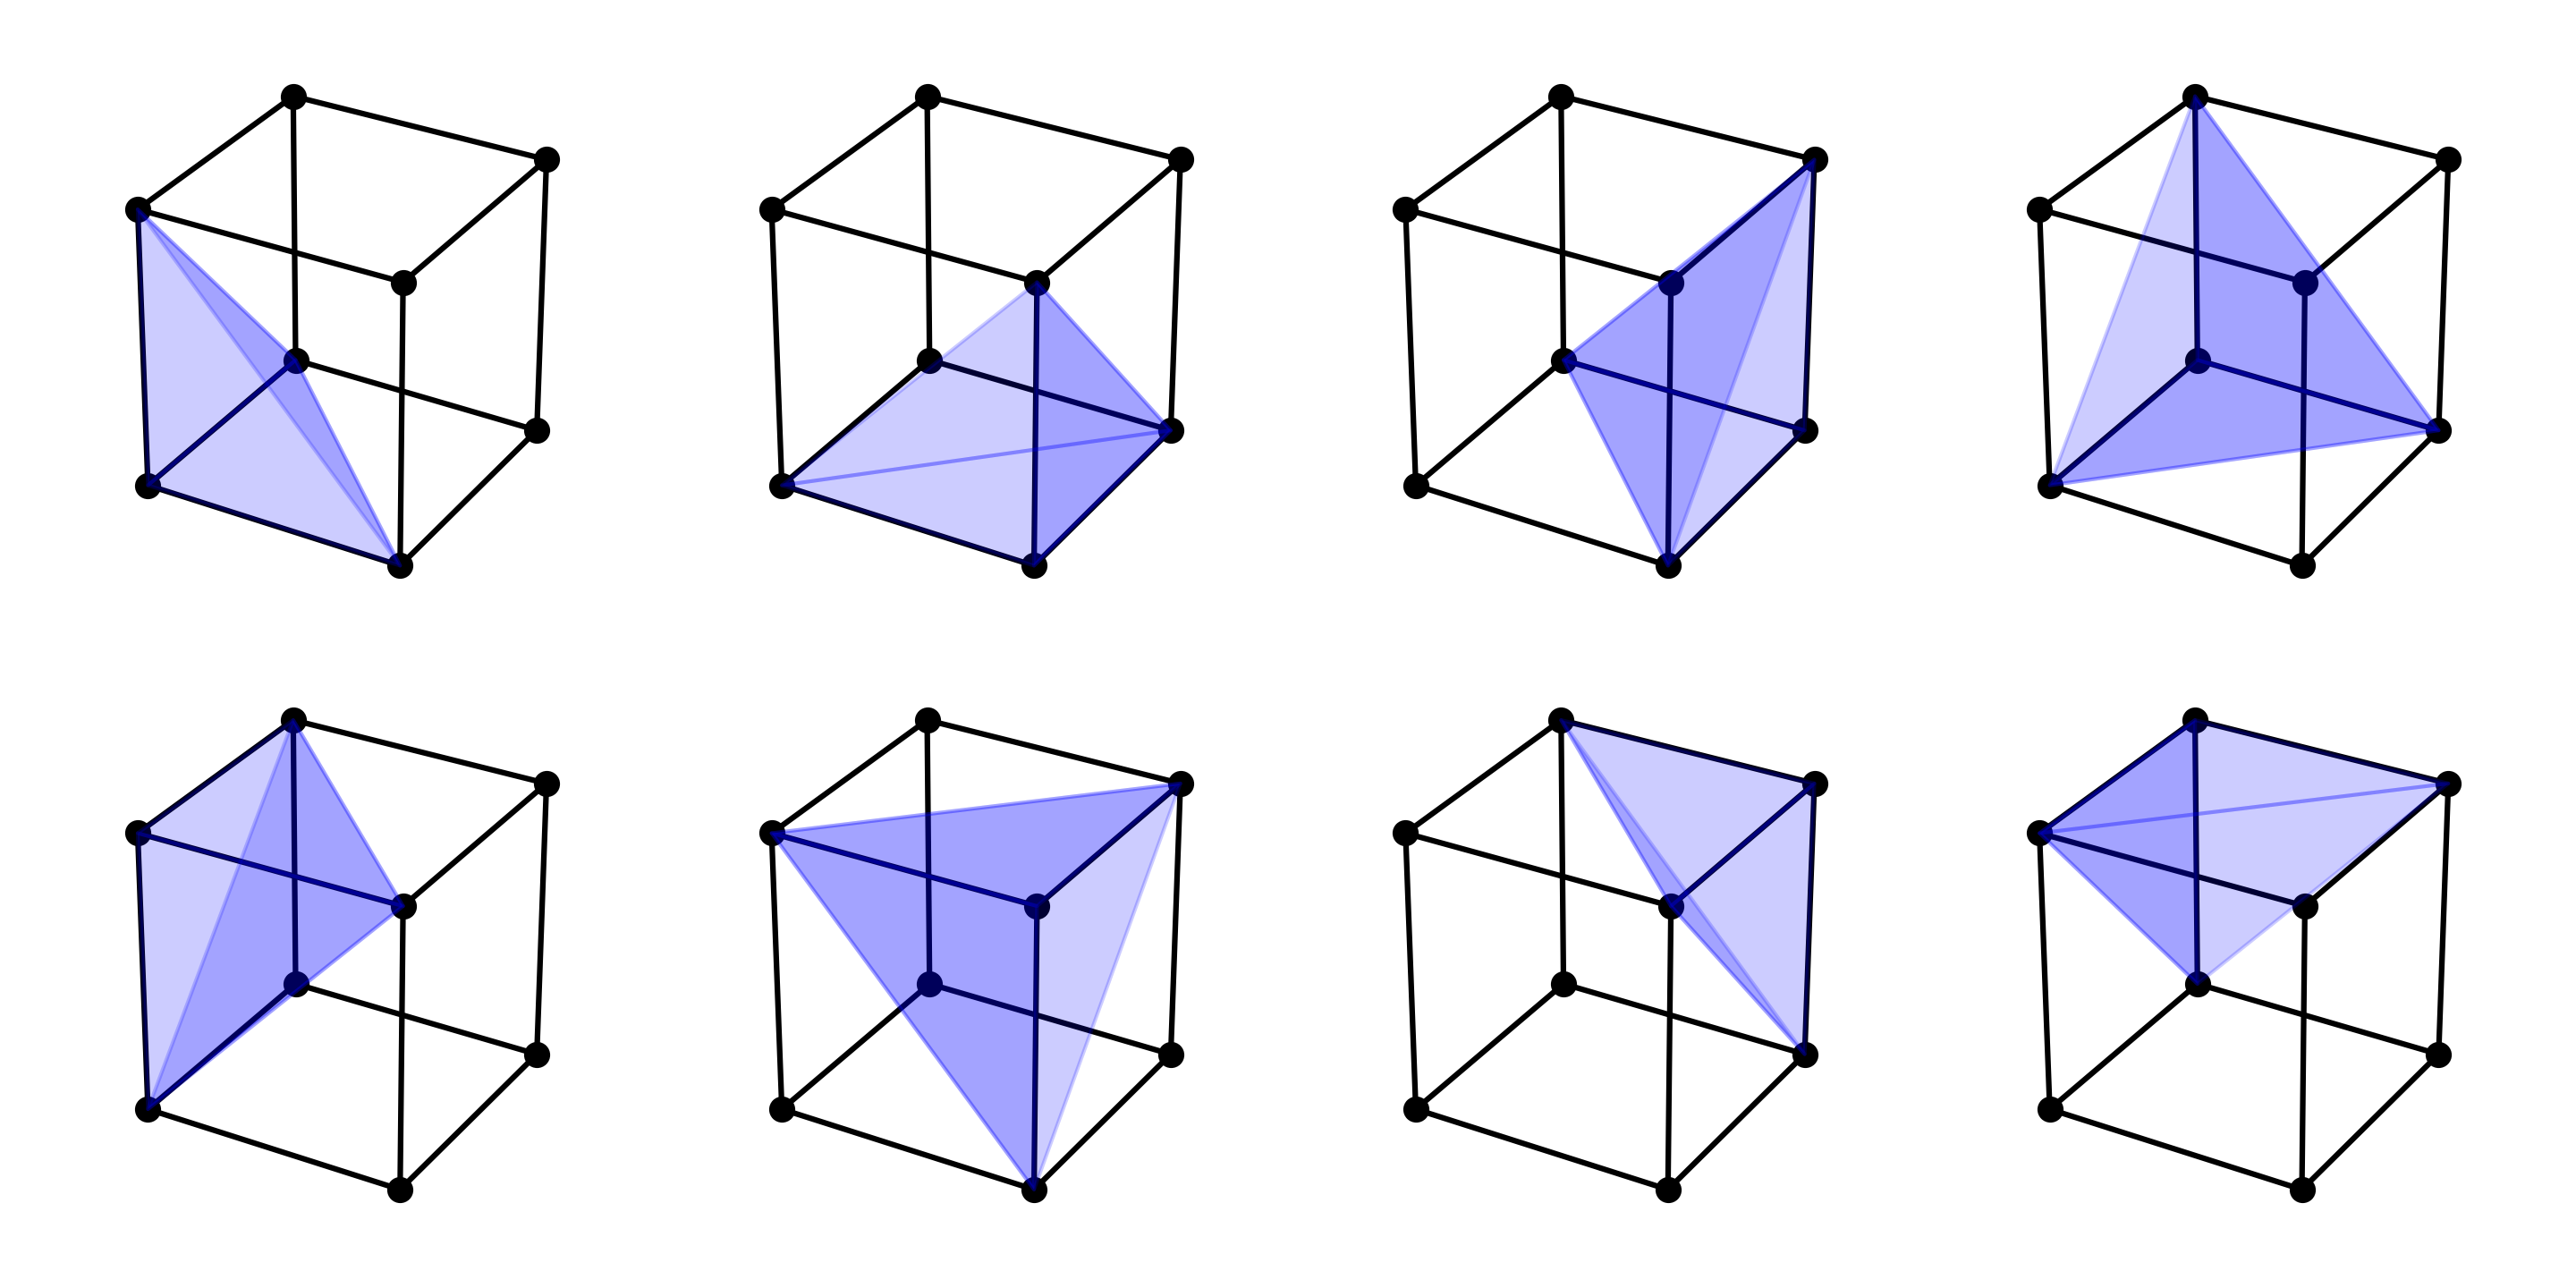
\includegraphics[width=0.4\textwidth]{../figs/one-tet-per-vertex.png}
    %\vspace{-0.35cm}
    %\caption{\label{fig:one-tet-per-vertex}
    %  \small
    %  Demonstration of one-per-vertex scheme.
    %}
  \end{figure}
\end{frame}